\documentclass[10pt]{beamer}

% Configuration {{{
\usepackage[utf8]{inputenc}
\usepackage[T2A]{fontenc} % T1 for English
\usepackage[english, russian]{babel}

\usepackage{mathtools}
\usepackage{graphicx}
\usepackage{tikz}
\usepackage[multidot]{grffile}
\usepackage[labelsep=period]{caption}
\usepackage{multirow}

\setbeamertemplate{caption}[numbered]
\setbeamertemplate{navigation symbols}{}
\usefonttheme[onlymath]{serif}
\usepackage{DejaVuSansCondensed} % helvet for English
\usetheme{Madrid}

\linespread{1.2}
% }}}

\title{``Сильная программа'' Блура}
\author{Керим Гусейнов}
%\institute[МГУ]{Московский государственный университет имени М.\,В.~Ломоносова}
\date{26 ноября 2022 г.}

\begin{document}

\frame[plain]{\titlepage}

\begin{frame}[label=pic]%{{{
  \frametitle{Дэвид Чарльз Блур (р. 1942)}

  Британский социолог, профессор и бывший директор отдела научных 
  исследований Эдинбургского университета.
  \vfill

  \parbox{.7\textwidth}{
    \small
    Работы:
    \begin{itemize}
      \item Знание и социальное представление.
      \item Витгенштейн. Социальная теория познания.
      \item Scientific knowledge: a sociological analysis.
      \item Toward a Sociology of Epistemic Things
      \item Epistemic Grace. Antirelativism as Theology in Disguise
      \item Ideals and Monisms: Recent Criticisms of the Strong Programme in the Sociology of Knowledge
      \item Relativism at 30,000 feet
      \item Relativism and the sociology of knowledge
    \end{itemize}
  } \hfill \parbox{.25\textwidth}{
    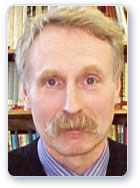
\includegraphics[width=\linewidth]{figures/Bloor}
    \vskip 2ex
    Коллеги:
    \\ Б. Барнс
    \\ Дж. Генри
    \\ М. Малкей
  }

\end{frame}%}}}

\begin{frame}[label=antropology]%{{{
  \frametitle{Антропология науки}

  Эволюция представлений об антропологии науки и развитие понимания 
  влияния человека на отношения субъект-объект происходит в философии 
  в несколько стадий:
  \begin{itemize}
    \item Классическая наука нового времени (17--19 века): творчество 
      ученого выводится за рамки научной рациональности. Дискуссии, 
      социальный, культурный, психологический аспекты научных открытий 
      -- лишь несовершенства.
      Бэкон, Беркли, Юм и др.
    \item 20 век: влияние квантовой механики, обращение исторических, 
      социальных, философских исследований к анализу субъекта как 
      к фактору научной деятельности, присутствующему в научной 
      рациональности и даже формирующему ее.
    \item Конец 20 века: еще большее внимание уделяется разным сторонам 
      исследования, помимо самого объекта. Распространение case-studies, 
      рассматривающих все событие-случай целиком.
  \end{itemize}
\end{frame}%}}}

\begin{frame}[label=overview]%{{{
  \frametitle{Общие черты ``сильной программы''}

  Эдинбургские социологи в рамках ``сильной программы'' анализируют 
  эпизоды в истории науки. Проблематика, понятия и методы исследования 
  объединяются у социологов, историков, философов. Рассматриваются 
  логические пристрастия ученых, личностные характеристики, цели, 
  намерения. Блур полагает, что эпистемологические факторы 
  в действительности являются социальными и что социологи помогают 
  раскрыть социальный характер эпистемологического.
  \vfill

  Сильная программа претендует на объяснение рациональных аспектов 
  научного знания. Именно это вызывает основную массу неприятия в ее 
  сторону.
\end{frame}%}}}

\begin{frame}[label=book1-1]%{{{
  \frametitle{Знание и социальное представление}

  Выдвигается натуралистическая программа социологии познания: сильная 
  программа. Блур переопределяет понятие знания -- то, что принимается 
  как знание людьми, конкретные убеждения. Не задается вопрос об их 
  истинности.
  \vfill

  Социологическое изучение познания должно привести к построению теории, 
  объясняющей закономерности распространения убеждений и причины их 
  возникновения.
\end{frame}%}}}

\begin{frame}[label=book1-2]%{{{
  \frametitle{Знание и социальное представление}

  Тезисы сильной программы:
  \begin{enumerate}
    \item Социология познания должна заниматься причинным объяснением 
      знания, хотя такое объяснение не исчерпывается социальными 
      причинами,
    \item Она должна объяснять все виды знания, оставаясь безразличной 
      к его истинности или ложности, рациональности или 
      иррациональности,
    \item Социологическое объяснение должно сводить истинное и ложное, 
      рациональное или иррациональное знание к одному типу причин 
      (принцип симметрии),
    \item Социология знания должна быть рефлексивной и применяться 
      к себе самой так же, как к другим системам знания.
  \end{enumerate}
\end{frame}%}}}

\begin{frame}[label=book1-3]%{{{
  \frametitle{Знание и социальное представление}

  Знание происходит как от опыта взаимодействия с материальным миром, 
  так и от социальных факторов одновременно. Оба фактора в ответе как за 
  истинность, так и за ложность знания. Блур говорит, что любое знание 
  имеет социальный компонент.

  \vfill
  Общество как архетип знания.
  Знание (научное и нет) обладает свойством сакральности 
  и рассматривается как отражение общественной идеологии: упрощенные 
  картины общества, которыми располагает субъект, находясь в этом 
  обществе. Блур считает идеологии источником и систем знания, 
  и философских представлений о природе знания. Говорит, что наблюдается 
  естественное сродство между обществом со всеми связями в нем 
  и знаниями его членов.
\end{frame}%}}}

\begin{frame}[label=book1-4]%{{{
  \frametitle{Знание и социальное представление}

  Конвенциональный элемент знания. Блур модифицирует миллевскую 
  эмпирико-психологическую теорию математического знания, вводя фактор 
  конвенциональности. Он обеспечивает социально поддерживаемый выбор из 
  всех возможных.

  \vfill
  Институционализированные посылки, принимаемые без доказательства 
  членами общества, не изменяются при столкновениях с логическими 
  противоречиями. Наличие таких посылок обусловлено конвенциональным 
  характером знания. Например, ими являются научные парадигмы, что 
  приводит к необходимости вводить гипотезы по мере надобности.

  \vfill
  Блур демонстрирует зависимость математического знания от культуры. 
  Исторически можно проследить различия как в когнитивных стилях 
  математической мысли, так и в значениях, придаваемых вычислениям, 
  импликациям, строгости рассуждений. Каждый из этих факторов у Блура 
  обусловлен социумом.
\end{frame}%}}}

\begin{frame}[label=book2-1]%{{{
  \frametitle{Витгенштейн. Социальная теория познания}

  Блур использует идеи позднего Витгенштейна, а свой анализ знания 
  основывает на материале из психологии, социальной антропологии 
  и истории науки. Блур стремится показать связь трудов Витгенштейна 
  с социологией познания, а также систематизировать его идеи. Знание 
  трактуется как коллективное поведение.

  \vfill
  Блур анализирует понятие значения, оно определяется общественными 
  практиками, и делает аналогичное утверждение о любом знании. Блур 
  строит свою теорию языковых игр, разрабатывая и уточняя Витгенштейна. 
  Он защищает институциональную природу сознания и говорит о зависимости 
  реакции человека от социального подкрепления.
\end{frame}%}}}

\begin{frame}[label=book2-2]%{{{
  \frametitle{Витгенштейн. Социальная теория познания}

  Касательно математики, Блур говорит о зависимости доказательства от 
  контекста его появления, включая цели и мыслительный подход. Блур 
  считает правдоподобие социологическим понятием и анализирует его 
  в этом свете.

  \vfill
  В конце концов, Блур строит компаративную теорию языковых игр 
  и утверждает, что принятый в обществе стиль поведения определяет 
  реакцию уже научного сообщества на аномалии и логические противоречия.
\end{frame}%}}}

\begin{frame}[label=summary]%{{{
  \frametitle{Заключение}

  \begin{itemize}
    \item Создается социальная эпистемология,
      \\ Знание объявляется зависимым от общественной конвенции,
    \item Отрицается эпистемологическая значимость науки,
      \\ Научное знание как совокупность соц. конструктов,
      \\ Объявляется подобным любым другим формам знания,
    \item В сильной программе Блура отрицание доходит даже до теории, 
      включая математику,
      %\\ Важно не уйти в скептицизм и агностицизм,
    \item Эволюция от первобытной магии до современной науки происходит 
      путем формирования убеждений, принятых в рамках определенной 
      социокультурной группы,
    \item Социологу поручается поиск теории, объясняющей фактически 
      существующие убеждения вне зависимости от каких-либо оценок этих 
      убеждений: дескриптивная установка.
  \end{itemize}
\end{frame}%}}}

\end{document}

% Антропология науки (Энциклопедия) {{{

АНТРОПОЛОГИЯ НАУКИ (от греч. anthropos — 
человек и logos — слово, понятие, учение) — понимание
науки и ее развития с точки зрения человеческого полюса
в познавательном отношении субъект—предмет. В 
классической науке Нового времени (17 — начало 20 вв.)
творческая деятельность ученого и сам ученый со всеми
его личностными характеристиками выводились за 
пределы научной рациональности. Научные дискуссии, 
социальный, культурный, психологический контексты 
научного открытия могли присутствовать в научном 
знании только как его недостатки, несовершенство. В 20 в.
положение дел существенно меняется, не в последнюю
очередь в результате трансформаций в самом
естествознании (принцип соответствия, принцип 
дополнительности в квантовой механике). Теории оборачиваются своей
субъектной стороной, на передний план выдвигаются
моменты их взаимоперехода, возникновения, роста. 
Соответственно исторические, философские, 
социологические исследования науки обращаются к анализу субъекта
как к такому фактору научной деятельности, который
в том или ином виде присутствует в самой научной 
рациональности и участвует в ее формировании. В 
интерпретациях науки ученый фигурирует как член или 
невидимого колледжа (Д. Прайс), или научного сообщества
(Т. Кун), или коллектива лаборатории (К. Кнорр-Цети-
на), или как одна из составляющих события в 
исследованиях типа «кейс стадис» (от англ. case studies — 
конкретное, ситуативное исследование — методика исследования
деятельности ученых, концентрирующаяся на анализе
конкретного примера) (П. Форман, Х.М. Коллинз).
Ученые в научном сообществе, работающие в русле
какой-то определенной парадигмы-теории, объединены
не только приверженностью к ней как к некоторой 
истине, но и множеством социальных, психологических, 
моральных обстоятельств. Научное сообщество 
принадлежит науке, вписывается в ее структуру, причем не только
социальную, но и логическую. Трудности, которые при
этом возникают, нашли свое отражение в дискуссиях о
соизмеримости парадигм, о релятивизме в науке, об 
истинности и объективности научного знания и т.д.
Ближе к концу 20 в. в истории науки происходит 
дальнейшая миниатюризация предмета исследования в связи
с распространением исследований типа «кейс стадис».
Для этих исследований важно, что в качестве целостного
и уникального берется событие, малое по объему: это не
наука в контексте культуры большого региона, а события
часто незначительные.
Эдинбургские социологи в рамках сильной программы
(Д. Блур и др.) в своих исследованиях науки базируются на
анализе именно отдельных эпизодов в истории науки.
В этом случае происходит совмещение проблематики, 
базовых понятий и методов исследования социологов, 
историков и философов науки. В рамках «кейс стадис» мы 
наблюдаем не только сосуществование логических, 
познавательных и нелогических, социальных в самом широком
смысле слова характеристик ученых (так было и в научном
сообществе), но пребывание в некоторой единой 
целостности исторического события, наряду с логическими 
пристрастиями ученых, их личностными характеристиками, а
также целями, намерениями, особенностями многих 
других действующих лиц. Все многообразие этих и прочих
социальных отношений вместе с логикой научного 
исследования формируют целостное событие-случай в истории
науки. «Кейс стадис» как определенный вид исторической
реконструкции упорно и настойчиво вторгаются в канву
рассуждений не только историков, но и социологов, 
философов. Существует целый набор «парадигмальных кейс
стадис», которые особенно часто используются для 
демонстрации концептуальных соображений.
Напр., Д. Блур (создатель сильной программы в 
социологии науки) с их помощью стремится обосновать свое
убеждение в том, что эпистемологические факторы в 
действительности являются социальными факторами, что
связь между предпосылкой и выводом социально 
конституирована. О тех исследователях, которые изучают
социальный фон эпистемологических процессов, 
нельзя сказать, полагает Блур, что они занимаются 
социальным, а не эпистемологическим, — нет, они помогают
показать социальный характер эпистемологического.
Оставаясь социологическим способом реконструкции
исторических событий, сильная программа тем не 
менее претендует на способность объяснить и 
рациональные аспекты научного знания. Именно это и вызывает,
в первую очередь, неприятие ее оппонентов.
В микросоциологии главным объектом исследования
становится лаборатория. Предполагается, что любое 
решение, принимаемое здесь, независимо от того, касается
оно методики проведения эксперимента или выбора 
поставщика экспериментального оборудования, в равной
мере участвует в формировании получаемого результата.
Социальные отношения в лаборатории формируют 
продукт науки. Социальность отождествляется с 
содержанием и логической структурой научного знания. Наиболее
бескомпромиссной в этих вопросах является позиция
К. Кнорр-Цетины. По словам Р. Харре, написавшего 
предисловие к ее книге, антропологический характер 
исследований состоит в том, что на лабораторию предлагается
смотреть взглядом путешественника в экзотические 
страны. Общества, обнаруженные здесь, наблюдаются 
человеком, принадлежащим совершенно к другой культурной
среде. Такой настрой ума заставляет исследователя 
увидеть лабораторию в необычном ракурсе. «По всей 
видимости, логика не принадлежит к числу "идолов племени". Там,
где она появляется, она становится чем-то вроде 
подспорья в риторических дебатах» (Knorr-Cetina К. D. The 
Manufacture of Knowledge. N.Y., 1981. P. VII). He существует 
никакой рациональности, специфичной именно для научной
деятельности, и нет никакой разницы между научным
и повседневным рассуждением. Ученый — это 
практический мыслитель, и различие «социальный/когнитивный»
устарело.
Если в научном сообществе и в «кейс стадис» 
предметом обсуждения остается знание и проблема его 
соответствия действительности, то в научной лаборатории 
логика рассуждений, постановка экспериментов, стремление
к истине, с точки зрения социолога, не заслуживают 
специального внимания. Профессионализм ученого и уме-64 • АНТРОПОМОРФИЗМ
ние хозяйственника обеспечить лабораторию всем 
необходимым равнозначны с точки зрения успеха в 
получении результата. Ученый — это, прежде всего, человек,
практикующий науку как способ жизни.
/I.A. Маркова

%}}}

% Витгенштейн: соц теория познания (Энциклопедия) {{{

«ВИТГЕНШТЕЙН: СОЦИАЛЬНАЯ ТЕОРИЯ 
ПОЗНАНИЯ» (BloorD. Wittgenstein: A Social Theory of 
Knowledge. Macmillan and Columbia, 1983.209 p.) — книга Д. Блу-
pa, представителя социальной эпистемологии 
(Эдинбургская школа). Блур придерживается дескриптивистской
позиции социологии познания и использует идеи 
позднего Л. Витгенштейна. Оставаясь на натуралистической по-ВНУТРЕННИЙ МИР, ВНЕШНИЙ МИР * 115
зиции, Блур наполняет свой анализ знания как 
социологического феномена эмпирическим (и теоретическим) 
материалом, взятым из психологии (К. Бюлер, Б. Скиннер), из
социальной антропологии (М. Дуглас), из истории науки.
Книга состоит из 9 глав. Целью исследования автор ставит
демонстрацию связи работ позднего Витгенштейна с 
социологией познания и систематизацию его идей. Знание
при этом трактуется как коллективное поведение, 
зависимое от паттернов обучения. Понятие знания как продукта
заменяется понятием познания как процесса — идея, 
плодотворная для современной эпистемологии.
В главе «От ментальных состояний к социальному
взаимодействию» Блур рассматривает критику 
Витгенштейном классических психологических теорий 
значения как ментального состояния (Э.Б. Тиченер, В. Вундт,
Б. Рассел) и ментального акта (Ф. Брентано). Здесь же
Блур анализирует дискуссию о «чистом мышлении» 
между Вюрцбургской психологической школой (О. Кюльпе,
Н. Ах, К. Бюлер) и такими психологами, как В. Вундт
и Э.Б. Тиченер (1900—1920). Блур подчеркивает 
сходство рассуждений Витгенштейна о «языковых играх»
с экспериментами Вюрцбургской школы.
В главе «Языковые игры и поток Жизни» Блур 
анализирует понятие значения, снова обращаясь к концепции
Витгенштейна: значение конституируется 
общественными практиками и является продуктом их 
конденсации. То же Блур утверждает о всяком знании, расширяя
коллективистический тезис. Витгенштейн использует
ряд конструкций — доктрина семейного сходства, 
отношения между критериями и симптомами, понятие 
потребностей, — которые он не конкретизирует 
достаточно подробно. Блур рассматривает каждую из этих 
конструкций, уточняя и применяя эти понятия в построении
своей теории языковых игр. Тезис об образовании 
понятий по принципу семейного сходства он 
иллюстрирует примерами из книги Л. Флека (Fleck L. Genesis and
Development of a Scientific Fact. Chicago, 1979).
В главе «Социальное конструирование ментальных
состояний» Блур защищает тезис об 
институциональной природе сознания. Он опирается при этом на 
позицию Б. Скиннера (см.: Skinner В. The Operational Analysis
of Psychological Terms (reprinted from the Psychological
Review. Vol. 52, 1942) // Feigl H, Brodbeck M. Readings in
the Philosophy of Science. N.Y., 1953), развивающего 
бихевиористскую теорию о зависимости реакций человека
(в том числе вербальных реакций и приватных 
ощущений как реакций, подобных другим) от социального
подкрепления. В главе «Математика как 
антропологический феномен» Блур выдвигает утверждение о 
зависимости смысла математического доказательства от 
контекста появления данного доказательства, 
включающего цели и применяемые мыслительные техники. В главе
«Принуждение, конвенция и кодификация» Блур 
рассматривает характер дедуктивных правил и 
анализирует происхождение и природу логической 
обоснованности. По Витгенштейну, принудительность дедуктивных
правил определяют обычаи, установленные в пределах
биологической структуры. Правдоподобие, по Блуру, —
типично социологическое понятие, и Блур анализирует
его как таковое. Развивая теорию языковых игр, Блур
вводит трехчастную модель доказательства в системе
знания: 1) интуиция; 2) существующие формальные 
системы; 3) интересы, относящиеся к использованию этих
двух факторов.
В главе «Систематическое изучение языковых игр» Блур
строит компаративную теорию языковых игр — цель всех
предыдущих исследований. При построении теории он
использует метод grid-group analysis, разработанный 
английским антропологом М. Дуглас. Два социальных 
измерения — внутригрупповая дифференциация и групповая
граница — служат М. Дуглас основаниями для 
классификации типов сознания разных социальных общностей.
Блур использует эту классификацию, защищая тезис о том,
что принятый в обществе социальный стиль определяет
реакции научного сообщества на аномалии и может 
служить для характеристики языковых игр (научных 
дискурсов). Блур использует также идею ограниченного набора
базисных стратегий ответа на аномалии, выраженную Ла-
катосом в его работах по истории математики (см.: Lakatos I.
Proofs and Refutations, the Logic of Mathematical Discovery/
Ed. J. Worrall and E. Zahar. Cambridge, 1976).
Принцип «социального использования природы», 
выделяемый Блуром, находится в зависимости от его тезиса
о множественности целей, достигаемых одной языковой
игрой. Социальная группа, строящая собственную 
картину мира, достигает по Блуру, одновременно как цели
построения такой картины, так и цели социального 
регулирования.
В главе «Позитивизм и культурный пессимизм» Блур
подчеркивает связь позиции Витгенштейна с 
консервативной традицией. Исследователь относит каждого 
рассматриваемого им философа (Л. Витгенштейн, П. Уинч,
Ю. Хабермас) к определенному типу, эксплицируя то,
в группе какого типа позиция мыслителя будет 
правдоподобной.
Книга Блура является одной из знаменательных 
попыток дальнейшего развития теории языковых игр 
позднего Витгенштейна и построения на ее основе 
компаративистской дескриптивистской социологии познания.
Ю.С.Моркина

%}}}

% Знание и социальное представление (Энциклопедия) {{{

«ЗНАНИЕ И СОЦИАЛЬНОЕ 
ПРЕДСТАВЛЕНИЕ» — книга Д. Блура представителя Эдинбургской
школы, в которой выдвинута натуралистическая 
программа социологии познания, которую автор называет
«сильной программой». В соответствии с принятой 
социологической точкой зрения, Блур переопределяет 
понятие знаниЯу предлагая изучать в качестве знания то,
«что принимается как знание людьми», т.е. конкретные
убеждения (beliefs), отвлекаясь от представления об их
истинности и ложности. Целью социологического 
изучения знания является построение теории, объясняющей
закономерности распространения убеждений и причины
их возникновения. «Сильная программа» социологии 
познания включает четыре тезиса (принципа):
1) социология познания должна заниматься 
причинным объяснением знания, хотя такое объяснение не 
исчерпывается социальными причинами,-
2) она должна объяснять все виды знания, оставаясь
безразличной к его истинности или ложности, 
рациональности или иррациональности;
3) социологическое объяснение должно сводить 
истинное и ложное, рациональное или иррациональное
знание к одному типу причин (принцип симметрии);
4) социология знания должна быть рефлексивной и
применяться к себе самой так же, как к другим системам
знания.
Точка зрения Блура на происхождение знания 
отличается дуализмом: в основе знания лежит 
материальный мир, порождающий опыт о нем, с одной стороны, и
социальный фактор, с другой. В соответствии с 
принципами «сильной программы» оба этих фактора 
симметричны по отношению к истинности или ложности
знания, определяемого ими. Как социолог Блур 
сосредоточивает свое исследование на втором факторе.
Любое знание, считает он, имеет социальный 
компонент. Книга представляет несколько моделей такого
компонента.
Представление об обществе как об архетипе 
знания. — Блур проводит параллель между собственным
рассмотрением знания и рассмотрением природы 
религии у Дюркгейма. Знание, в первую очередь научное,
обладая свойством сакральности, может 
рассматриваться как отражающее общественные идеологии, т.е.
те упрощенные картины общества, которыми 
располагает субъект в данном обществе. Примерами 
идеологий, рассматриваемых Блуром, являются 
Просвещенческий и Романтический взгляды на мир, 
противостояние которых отразилось, в частности, в различии
теорий познания у К. Поппера и Т. Куна. Блур считает
идеологии первоисточником как систем знания, так и
философских представлений о природе знания; он 
видит «естественное сродство» между представлениями
об обществе и его связях и представлениями о знании,
эксплицируемыми членами данного общества.
Представление о конвенциональном элементе 
знания. — Выражением «натуралистического взгляда на 
математику» является модификация Блуром миллевской
эмпирико-психологической теории математического 
знания путем введения фактора конвенциональности, 
обеспечивающего социально поддерживаемый выбор из 
возможных математических операций, а также 
объективность и принудительность математического знания.
Наличие институционализированных посылок, 
принимаемых без доказательства членами общества и не 
изменяемых при столкновении их с логическими 
противоречиями. — Примерами таких посылок Блур считает
конвенционально принимаемые научные парадигмы, 
неизменность которых приводит к необходимости введения
гипотез ad hoc.
В качестве образца знания для демонстрации 
социологического подхода Блур выбирает математику — науку,
система знания которой считается самой 
принудительной — и демонстрирует культурозависимость 
математического знания. Он полагает, что исторически можно
проследить различия как в когнитивных стилях 
математической мысли, так и в значениях, придаваемых 
вычислениям, импликациям, строгости рассуждений: каждый
из этих факторов Блур представляет как социально 
обусловленный.
Ю.С. Моркина

%}}}

% Социальная эпистемология. Социальность познания (Энциклопедия) {{{

Социальная эпистемология

Социальность познания

Блур добавляет, что социологическая дефиниция 
знания «будет поэтому отличаться от обыденного или 
философского его понимания. Вместо того чтобы определять
его как истинное убеждение, социолог рассматривает как
знание то, что является таковым в реальной человеческой
жизни» (Bloor D. Knowledge and Social Imagery. L., 1976.
P. 2). Это означает, что «социолог ищет теории, которые
объясняют фактически существующие убеждения 
независимо от того, как сам исследователь оценивает их»
(Ibid. P. 3). «Исходным для социального анализа 
знания, — пишет X. Новотни, — является тот факт, что у 
людей имеются весомые социальные основания для того,
чтобы придерживаться данных представлений и 
убеждений, коллективно отстаивать их и относиться к ним как к
знанию... Хотя с некоторых пор мы привыкли 
приписывать научному знанию верховный социальный и 
эпистемологический статус, к которому добавляется 
привилегия судить о правоте других убеждений, было бы все же
большим упрощением отбрасывать как иррацональное,
эмоциональное и необоснованное всякое явление, к 
которому не приложимы стандарты научной рациональности.
Допуская иные, социальные стандарты в качестве 
правомерных, социолог смотрит на науку как на социальный 
институт и на знание как на социальную конструкцию»
(Nowotny К Science and Its Critics//Counter-movements in
Science. Dordrecht, 1979. P. 5). Данные исследователи едины
в своей феноменологически-дескриптивисткой установке,
солидаризируясь с Витгенштейном в том, что разные 
формы знания следует изучать как обычаи примитивного
племени и, уподобляясь этнографу, заниматься их 
описанием, а не оценкой. Однако такое описание на деле 
выливается в реконструкцию, когда, напр., микросоциологи
представляют познавательный процесс как «социальное
конструирование» (социальное производство) знания.

%}}}

% Эпистемологическая значимость науки (Энциклопедия) {{{

ЭПИСТЕМОЛОГИЧЕСКАЯ 
ИСКЛЮЧИТЕЛЬНОСТЬ НАУКИ — тезис, согласно которому знания,
вырабатываемые в науке, обладают выделенным 
статусом, т.е. по своей обоснованности, достоверности, 
доказательности и т.п. качественно отличаются от всех др.
видов и форм знания. Явное или неявное принятие
этого тезиса — необходимое предварительное условие
для постановки «проблемы демаркации», 
предполагающей в рамках эпистемологии, философии науки и
социологии науки поиск тех особенностей научного
знания или социальной организации науки, которые
обеспечивают особый статус научного знания.
В классической эпистемологии этот тезис 
обосновывался наличием особых методов получения 
достоверного знания, характерных для науки, а также 
представлением о том, что научное знание в отличие от др.
видов знания опирается на надежные основания и 
источники (эпистемологический фундаментализм). 
Резко подчеркивали данный тезис представители 
логического эмпиризма, по сути отрицавшие познавательную
значимость всех видов и форм знания за исключением
науки и здравого смысла.
Утверждение об Э. и. н. стало подвергаться 
критическому анализу начиная с 1960—70-х в рамках 
исторической школы в философии науки (П. Фейерабенд), а
также в социально-конструктивистских направлениях
в философии и социологии науки. Отказ от положения
о том, что «наука представляет собой особый 
эпистемологический, а значит, и социологический случай»
(Малкей М. Наука и социология знания. М., 1988. С. 32),
приводит к пониманию научного знания как всего
лишь совокупности социальных конструктов, 
порождаемой взаимодействием людей в рамках социального
института науки и принципиально ничем не 
отличающихся от любых др. форм знания. Так, по словам
Б. Барнса, «естествознание не обладает специальным
статусом как объект социологического исследования, а
его мнения обнаруживают те же ссылки на принятые
стандарты, что и идеология примитивного мышления»
{Bûmes В. Scientific Knowledge and Sociological Theory.
L., 1974. P. 43). Взаимодействие исследователей с 
познаваемыми объектами в процессе получения 
эмпирических данных, оказывается при таком подходе чем-то
несущественным, вторичным. Тем самым, вместо 
поиска решения большого круга проблем философии 
науки, относящихся к обоснованности, проверяемости и
доказательности эмпирического содержания науки, по
существу отрицается их значимость. В более 
радикальных версиях социологии знания (напр., в «сильной 
программе» Д. Блура) аналогичным образом отрицается
особый эпистемологический статус теоретических 
высказываний науки, включая положения математики.
Б.Г.Юдин

%}}}

% Выдержка из разных мест (Энциклопедия) {{{

Выбор теории --- ... ---
На современном этапе возможность разрешения 
ситуации выбора на когнитивной основе отрицают 
социальные конструктивисты (Б. Латур, С. Вулгар), 
утверждающие, что научные факты являются социальными
конструкциями, в связи с чем В. т. не может быть 
квалифицирован как рациональная процедура, а также 
сторонники «сильной программы» социологии познания
(Д. Блур, Б. Барнс, С. Шейпин), утверждающие, что
оценка и В. т. определяются социальными факторами,
так что сама процедура выбора должна быть объектом
не когнитивного, а социологического анализа.

Заблуждение --- ... ---
Методы социального конструирования оказались 
востребованы в социологии научного знания, начиная со 
второй половины 1970-х, и при этом как в экстерналистском
(Б. Варне, Д. Блур), так и интерналистском (Б. Латур,
С. Вулгар, К. Кнорр-Цетина) направлениях данной 
дисциплины. В первом из них конструирование 
когнитивных феноменов от первобытной магии до современной
науки строилось в форме их редукции к набору 
убеждений и верований («социальных образов»), принятых
в рамках некоторой социокультурной группы и 
выражающих собой ее основные параметры (внешнюю 
границу и внутреннюю структуру, по М. Дуглас).

Конструктивизм --- ... ---
Методы социального конструирования оказались 
востребованы в социологии научного знания, начиная со 
второй половины 1970-х, и при этом как в экстерналистском
(Б. Варне, Д. Блур), так и интерналистском (Б. Латур,
С. Вулгар, К. Кнорр-Цетина) направлениях данной 
дисциплины. В первом из них конструирование 
когнитивных феноменов от первобытной магии до современной
науки строилось в форме их редукции к набору 
убеждений и верований («социальных образов»), принятых
в рамках некоторой социокультурной группы и 
выражающих собой ее основные параметры (внешнюю 
границу и внутреннюю структуру, по М. Дуглас).

"Наука и социология знания" --- ... ---
Более того, в так называемой «сильной программе 
социологии знания» Д. Блура (Bloor D. Wittgenstein and
Mannheim on the sociology of mathematics // Stud. Hist.
And Philos. Sei. Studies in History and Philosophy of Science.
1973. Vol. 4. #2. P. 173—191), как и в ряде др. 
радикальных концепций, уже сама по себе когнитивная сторона
научного познания выступает в качестве некоего 
эпифеномена. С точки зрения Д. Блура, социолог должен
быть в состоянии объяснить из социальных условий
возникновение любых верований безотносительно к их
оценке с точки зрения истинности. Иными словами, не
следует даже задаваться вопросом об истинности тех
или иных утверждений как таковых (включая, в частно-
сти, и законы логики и математики), — вопрос в том, 
каковы социальные механизмы, под действием которых
мы признаем эти утверждения истинными либо 
ложными.

Case studies как альтернатива методу рациональной реконструкции Поппера.

Социология знания ---
Социальное конструирование и реальности, и знания.

Социология науки ---
Особенностями когнитивной С. н. являются: 1) анализ
научного знания как особой системы убеждений; 2) 
обращение к социологическому причинному объяснению
когнитивных форм убеждений и содержания научного
знания; 3) преимущественное внимание к 
псевдоэффектам в науке, не получившим признания (парапсихология,
френология, различные псевдоэксперименты, 
«опровергающие» теорию относительности и квантовую 
механику); 4) выдвижение в качестве основания С. н. интереса
ученых, который обеспечивает конструирование знания
из доступных культурных ресурсов; 5) трактовка его 
содержания как эпифеномена социальных интересов; 6) 
поворот к анализу дискурса, который включает в себя как
изучение исследовательских статей, так и интервью с 
учеными; 7) фиксация несовместимости убеждений 
различных исследовательских групп, что находит свое 
выражение в альтернативности как их интерпретационных схем,
так и эмпирических фактов, конструируемых в ходе 
теоретических интерпретаций; 8) преимущественный 
интерес к микросообществам и к микроанализу «отдельных
случаев».
---
Наряду с «сильной программой» в С. н. (Блур), 
основными принципами которой являются каузальность, 
беспристрастность, рефлексивность (С. н. должна 
применять эти требования и к самой С. н.) и симметрия в
объяснении социальных причин как истинного, так и
ложного знания, ...

Философия науки ---
Авторы «сильной 
программы» в когнитивной социологии науки (Б. Барнс, Д. Блур)
раскрывают макросоциальные механизмы производства
знания из социальных ресурсов.

%}}}

% Выдержка из лекции Хмелевской {{{
  Локк, Юм, Т. Рид?.
  Маркс, Маннгейм?, Франкфуртская школа и Хабермас?.
  + Богданов...
  + Кун с парадигмой...
  + Фуко археология знания...

  Современные направления:
    Консервативное («веритистское», используя термин Э.Голдмана):
    - классические допущения о центральности для эпистемологии понятий 
      «истина»;  эпистемической рациональности;
    - эпистемика Э.Голдмана; социальная эпистемология науки Ф.Китчера;
    Радикальное (социально-конструктивистское):
    - социальная детерминация и социально-историческая релятивность 
      убеждений любого вида;
    - Эдинбургская школа: Д.Блур, Б.Барнс; Б.Латур; Г.Коллинз

  - Антиреализм: научное знание сконструировано учеными, а не 
  детерминировано действительностью.
  - Формирование убеждений в науке столь же подвержено социальным 
  влияниям, как и формирование убеждений во всех прочих областях 
  социальной жизни.
  - Истинность или ложность определяются социальными интересами 
  и социальной структурой данного научного сообщества.

%}}}


  -----

  Почему так называется: сильная программа?
  Своя собственная теория истины?

  -----

  Энциклопедия: стр. 114, 250, something at 900


=============================================================

Социальная эпистемология. В ней есть радикальный конструктивизм.


 «полевые» (этнографические) социологические исследования науки; 
 «сильная» программа    когнитивной социологии (К. Кнорр-Цетина, Д. 
 Блур); отрицание объективности особого эпистемологического статуса 
 науки; понятия институционального и континджентного форумов науки
